\documentclass[12pt]{report}

%Packages-------------------------------------
\usepackage{amsmath}
\usepackage{amsfonts}
\usepackage{amssymb}
\usepackage{amsthm}
\usepackage{graphics}
\usepackage{graphicx}
\usepackage{float}
\usepackage{adjustbox}
 \usepackage[stable]{footmisc}
\usepackage{setspace}
\usepackage{adjustbox}
%\usepackage{hyperref}
\usepackage{pgfplots}
%\usepackage{xtocnic}

\usepackage{listings}
\usepackage{caption}
\usepackage{xepersian}

\lstset{
basicstyle=\small\ttfamily,
columns=flexible,
breaklines=true
}
\settextfont{XB ZAR.TTF}
\renewcommand\bibname{مراجع}


%Layout---------------------------------------

%\usepackage[top=2cm, bottom=2cm, left=2cm, right=2cm]{geometry}

%Commands-------------------------------------


%Theorems-------------------------------------

\begin{document}

%Title page ---------------------------------------------

\begin{figure}
\centering
\includegraphics[height=2.5cm]{UT-Logo.pdf}
\end{figure}

\begin{center}
پردیس علوم
\\
دانشکده‌ی ریاضی، آمار و علوم کامپیوتر
\end{center}

\begin{center}
%%%%%%%%%%%%%
\end{center}

\begin{center}
\huge{ تحلیل داده‌های بازار بورس ایران با استفاده از الگوریتم‌های داده‌کاوی}
\end{center}

\begin{center}
%%%
\end{center}

\begin{center}
نگارنده
\end{center}
\begin{center}
\textbf{
محمدحسین خوش رفتار 
}
\end{center}

\begin{center}
\begin{tabular}{rr}
استاد راهنما: دکتر سمانه افتخاری مهابادی
\end{tabular}
\end{center}

\vspace{3cm}
\begin{center}
پایان‌نامه برای دریافت درجه کارشناسی
\\
در رشته علوم کامپیوتر
\end{center}

\begin{center}
تیر ۱۴۰۰
\end{center}

\pagestyle{empty}
\pagenumbering{}

\newpage
%\pagestyle{headings}
%\setcounter{page}{1}
%\pagenumbering{roman}
\pagestyle{plain}
\setcounter{page}{1}
\pagenumbering{harfi}
%Abstract page-------------------------------
\doublespacing{}
\chapter*{}
\section*{چکیده}
هدف این پروژه پیش بینی وضعیت سهم های بازار بورس تهران با استفاده از تاریخچه ی سهم و سایر شاخص های اقتصادی از جمله قیمت دلار ، تورم ، نقدینگی و … میباشد. با استفاده از روش ها و الگوریتم های داده کاوی سعی کردیم که به کمک تاریخچه ی سهم و شاخص های اقتصادی مهم به مدلی دست پیدا کنیم که آینده ی سهم را پیش بینی کند. در گام نخست دیتای مورد نیاز راجمع آوری کردیم. دیتای سال ۲۰۱۵ تا سال ۲۰۲۰ تمامی سهم ها و شاخص های اقتصادی نام برده شده را با فرمت csv ذخیره کردیم. در گام بعدی با رسم نمودار های مناسب و تحلیل شاخص ها کنار هم به بررسی اینکه کدام شاخص ها بر قیمت سهم تاثیر گذارند پرداختیم و شاخص های مناسب را انتخاب کردیم. در گام آخر هم با استفاده از دیتای موجود به بررسی و تست مدل های مناسب جهت پیش بینی سری های زمانی با دقت مناسب پرداختیم و در نهایت با استفاده از 
مدل میانگین متحرک خود همبسته یکپارچه
\footnote{\lr{ARIMA model}}
یک مدل جهت پیش بینی قیمت سهم ها آموزش دادیم و دقت سنجی کردیم.

\chapter*{پیشگفتار }


مهم ترین مسئله تو بازار سرمایه پیشبینی آینده سهم است. با مشخص شدن وضعیت سهم تو آینده ، استراتژی خرید و فروش به آسانی به دست می آید و می توانیم میزان سود را ماکزیمم کنیم. فاکتور های بسیار زیادی بر قیمت سهم تاثیر گذار هستند. مهم ترین فاکتور ها عملکرد مالی شرکت صاحب سهم و تاریخچه ی خود سهم هستند ولی از آنجایی که در کشور وضعیت شاخص های اقتصادی پایدار نیست ، عواملی چون قیمت دلار ، تورم ، نقدینگی و … تاثیر قابل توجهی روی قیمت سهم ها می گذراند. ازینرو برای پیش بینی قیمت سهم نیازمند مدلی هستیم که علاوه بر توجه به تاریخچه ی سهم یا همان ویژگی های سری های زمانی به تاریخچه ی دیگر شاخص های اقتصادی نیز توجه نماید و تغییرات آن ها را در تصمیم گیری لحاظ کند. یکی از چالش های مهم تو این راه این است که واحد ها و مقیاس های موارد مطرح شده یکسان نمی باشد و این موضوع باعث ایجاد بایاس در مدل و تصمیم گیری خواهد شد که باید با استفاده از نرمال سازی و تبدیل های مناسب این مشکل را برطرف کرد
\tableofcontents


\chapter{مقدمه}

\pagestyle{plain}
\setcounter{page}{1}
\pagenumbering{arabic}
پروژه از ۳ فاز اصلی تشکیل شده که به ترتیب جمع آوری و پیش پردازش دیتا، بررسی شهودی و انتخاب پیشگو ها و در نهایت طراحی و پیاده سازی مدل می باشد.
تمام مراحل فنی این پروژه با استفاده از
زبان برنامه نویسی پایتون
\footnote{\lr{Python programming language}}
 پیاده سازی شده است و تمام مراحل پیاده سازی پروژه تحت
 گیت
\footnote{\lr{Git}}
ثبت شده است و میتوانیم مراحل و تاریخچه را به کمک آن ببینیم.
به منظور تصمیم بهتر راجع به
پیشگو
\footnote{\lr{Predictor}}
های اقتصادی مطرح شده لازم داریم به طور شهودی با آن ها آشنا باشیم که در ادامه به طور مختصر توضیحاتی راجع به آن ها فراهم شده است. 
علاوه بر این نیازمند برای فهم بهتر تحلیل های ارائه شده خوب است که با مفاهیم اولیه ی بازار بورس آشنا باشیم ولی به دلیل گستردگی این مطالب از اشاره به همه ی آن ها  در این مقاله  خودداری کرده ایم و فقط به موارد ضروری اشاره کرده ایم

\section{مفاهیم}
\subsection{قیمت دلار}
در این پروژه منظور از قیمت دلار ، ارزش یک دلار آمریکا به ریال در تاریخ مشخصی و با توجه به قیمت رسمی اعلام شده از سوی بانک مرکزی می باشد.
\subsection{تورم
\footnote{\lr{Inflation}}
}
 از نظر علم اقتصاد اشاره به افزایش سطح عمومی تولید پول، درآمدهای پولی یا قیمت است. تورم عموماً به معنی افزایش غیرمتناسب سطح عمومی قیمت در نظر گرفته می‌شود. تورم، روند افزاینده و نامنظم افزایش قیمت‌ها در اقتصاد است. هر چند بر پایهٔ نظریه‌های گوناگون، تعریف‌های متفاوتی از تورم ارائه می‌شود، اما، تمامی آن‌ها به روند فزآینده و نامنظم افزایش در قیمت‌ها اشاره دارند.
 در این پروژه از آمار رسمی که توسط سازمان آمار اعلام می شود و بر اساس میانگین افزایش قیمت کالا محاسبه میشود استفاده شده است.
\subsection{نقدینگی
\footnote{\lr{Cash}}
}
منظور از نقدینگی، میزان سرمایه ی نقدی که دست مردم است می باشد. این سرمایه شامل اعتبار حساب بانکی افراد ، پول نقد در دسترسشون، و یا دیگر سرمایه های نقدی مردم می شود . باید توجه داشت که خودرو ، مسکن و یا دلار جز سرمایه های نقدی افراد حساب نمیشود و جز آمار نقدینگی محسوب نمیشود چون با نقد شدن مقداری فاصله دارد.
در این مقاله از آمار رسمی بانک مرکزی راجع به نقدینگی استفاده شده است.
\subsection{تاریخچه قیمت
\footnote{\lr{Price history}}
}
منظور از تاریخچه ی قیمت، 
سری زمانی 
\footnote{\lr{Time series}}
قیمت سهم می باشد. یعنی اینکه به ازای هر روز خاص قیمت سهم تو اون روز چقدر بوده است.

\subsection{قیمت پایانی
\footnote{\lr{Closing price}}
}
منظور از قیمت پایانی یک روز، میانگین وزن دار تمام معاملات آن روز با وزن حجم معاملات انجام شده می باشد
\chapter{مراحل فنی پروژه}

\section{جمع آوری و پیش پردازش دیتا}
برای هر نوع تحلیل داده کاوی ما نیازمند دیتا هستیم. بدون دیتا هیچ تحلیلی هم امکان پذیر نیست. همچنین این دیتا می بایست یک سری ویژگی ها داشته باشد که تحلیل ما را آسان تر و دقیق تر بکند.
\subsection{جمع آوری دیتای بورس}
برای تحلیل  ما نیازمند تاریخچه ی سهم های بازار بورس ، تاریخچه ی قیمت دلار ، تورم و نقدینگی بودیم. برای دسترسی به دیتای تاریخچه ی سهم های بازار بورس راه های فراوانی هست و ما از کتابخانه ی پاتونی
pytse\_client 
استفاده کردیم که قابلیت دانلود تاریخچه ی تمام سهم های بازار سرمایه را به ریزدانگی روز از سال ۲۰۱۵ را در اختیارمون قرار میدهد. خروجی استفاده از این کتابخانه یک فایل csv به ازای هر سهم بازار می باشد که حاوی تاریخچه ی سهم مورد نظر با ریزدانگی روز می باشد.
این فایل ها در پوشه ی tickers\_data از پروژه قرار دارند.
 به این نکته توجه شود که قیمت پایانی سهم به عنوان قیمت اون روز سهم در نظر گرفته شده است.
\subsection{جمع آوری دیتای شاخص های اقتصادی}
برای جمع آوری دیتای تاریخچه ی قیمت دلار از 
منبع شبکه ی اطلاع رسانی قیمت ارز
\footnote{\lr{tgju}}
استفاده شد و قیمت دلار به صورت ماهانه در فایل با فرمت csv ذخیره گردید.
برای سایر شاخص های اقتصادی نام برده شده از منبع مرکز آمار و بانک مرکزی استفاده گردید و دیتای ماهانه ی شاخص های مذکور در فایل با فرمت csv با اسامی مشخص هر شاخص ذخیره گردید که در ادامه مورد استفاده قرار گیرد.

\subsection{ حذف نوسانات مقطعی دیتا}
در گام نخست به منظور ساده تر شدن تحلیل و حذف نوسان های مقطعی به پیشنهاد استاد سطح ریزدانگی داده را از روزانه به ماهانه تغییر دادیم بدین شکل که به ازای هر سهم و یا شاخص اقتصادی به جای اینکه به ازای هر روز قیمت را نگه داریم به ازای هر ماه قیمت ابتدا یا انتهای آن ماه رانگهداری کنیم و بر اساس این دیتا تحلیل رو انجام دهیم. 


\subsection{
رسیدگی به داده های 
گم شده
\footnote{\lr{Missing data}}
}

با توجه به اینکه نماد های بازار بورس  بر اثر افشا ها یا سایر موارد ممکن است روز هایی بسته باشند و دیتا اون روز ها موجود نباشد ، ممکن است در تحلیل ها ما را دچار مشکل کنند و این مسئله باید رسیدگی شود. ازین رو از روش 
آخرین مشاهده انجام شده به جلو
\footnote{\lr{last observation carried forward}}
برای پر کردن جای خالی این روز ها استفاده کردیم. بدین شکل که قیمت اولین روزی که سهم بعد از بسته بودن باز شده و تعیین قیمت شده است را به جای روز های بسته بودن سهم قرار می دهیم

\subsection{یکسان سازی مقیاس ها}
با توجه به اینکه مقیاس سهم های بازار سرمایه ، قیمت دلار و سایر شاخص های اقتصادی تفاوت بسیار زیادی دارد و این تفاوت در مقیاس باعث ایجاد خطا در تحلیل ها و همچنین خراب کردن عملکرد مدل می شوند به پیشنهاد استاد به جای استفاده از مقدار متغییر ها از درصد تغییر شاخص ها برای تحلیل استفاده کردیم. درصد تغییر در سهم های بازار بورس به همان معنی بازدهی ماهانه سهم هستند و در سایر شاخص ها هم درصد تغییر شاخص در ماه مورد نظر هستند.
\subsection{یکسان سازی مولفه ی x دیتا}
روشی که ما برای رسیدگی به داده های گم شده انتخاب کردیم باعث میشد که مولفه ی x دیتای ما که از جنس تاریخ بود در بهضی از ماه ها یکسان نباشد بدین شکل که در حالت عادی روز اول ماه هست ولی در حالتی که جای گذاری اتفاق افتاده روز دوم سوم یا جلوتر از ماه باشد و این تفاوت در مرحله ی پیاده سازی مدل برامون مشکلاتی به وجود آورد برای همین به جای نگهداری روز در مولفه ی x دیتامون مستقیما ماه مورد نظر رابه عنوان مولفه ی  x در نظر گرفتیم. به طور مثال تاریخ 2019-04-03 به 2019-04 تغییر کرد

\section{تحلیل پیشگو ها}
اکنون که دیتا آماده و تمیز شده است نیازمند این هستیم که پیشگو هایی که انتخاب کرده ایم را بررسی نماییم تا از بین پیشگو های مورد نظر فقط آن هایی که در متغییر هدف ما تاثیر گذار هستند  را به مرحله ی طراحی مدل ببریم. لازم به ذکر است که تاریخچه ی خود سهم با توجه به شناختی که از دیتا داریم پیشگویی اجتناب ناپذیر می باشد و بدون تحلیل به مرحله مدل سازی میبریم. از ابزار های شهودی آمار جهت تحلیل پیشگو ها استفاده کردیم. به منظور رسم نمودار های مورد نیاز از کتابخانه ی پایتونی matplotlib استفاده کردیم.

\subsection{بررسی تاثیر قیمت دلار}
از بین سهم های بازار بورس نماد های فولاد، اخبار و خودرو را به نمایندگی از شاخص های بزرگ جهت تحلیل انتخاب میکنیم.
ابتدا
نمودار اسکتر 
\footnote{\lr{Scatter plot}}
قیمت دلار را در کنار سهم های مذکور مورد بررسی می نماییم.
\begin{figure}[H]
\centering
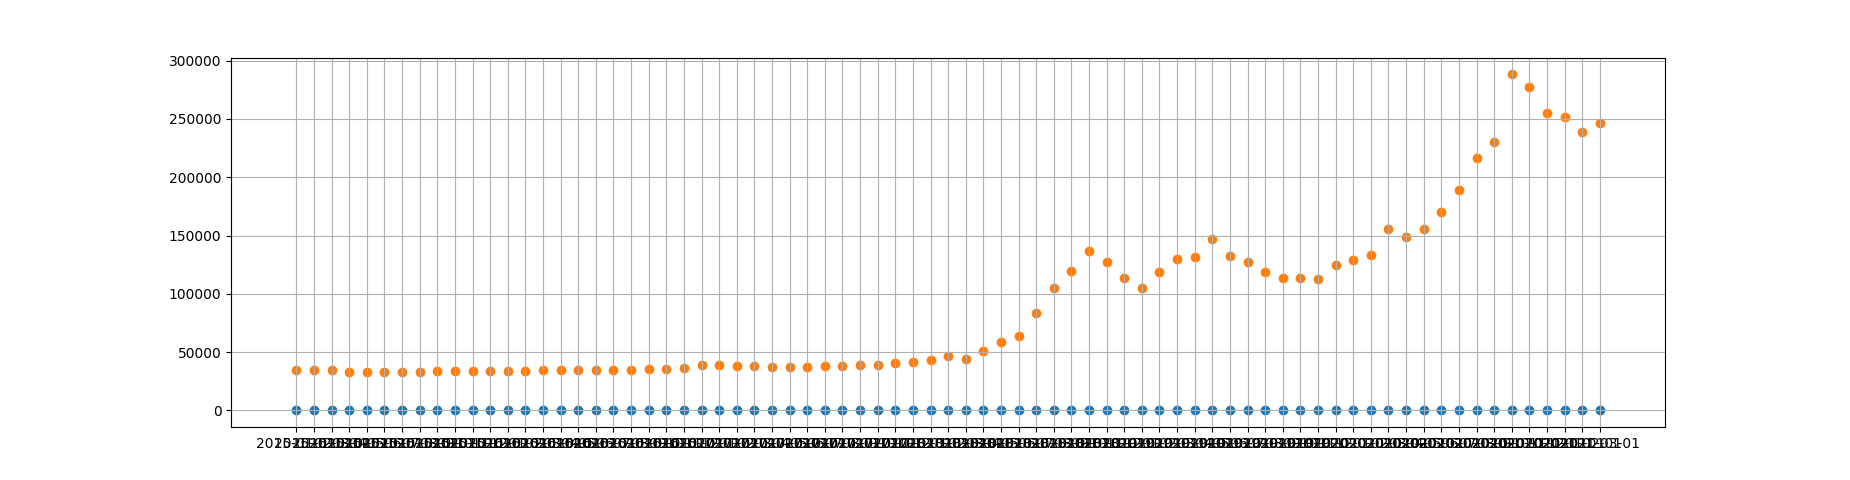
\includegraphics[width=1\textwidth] {dollar.png}
\label{dollar}$•$
\caption{
نمودار قیمت دلار
}
\end{figure}
\begin{figure}[H]
\centering
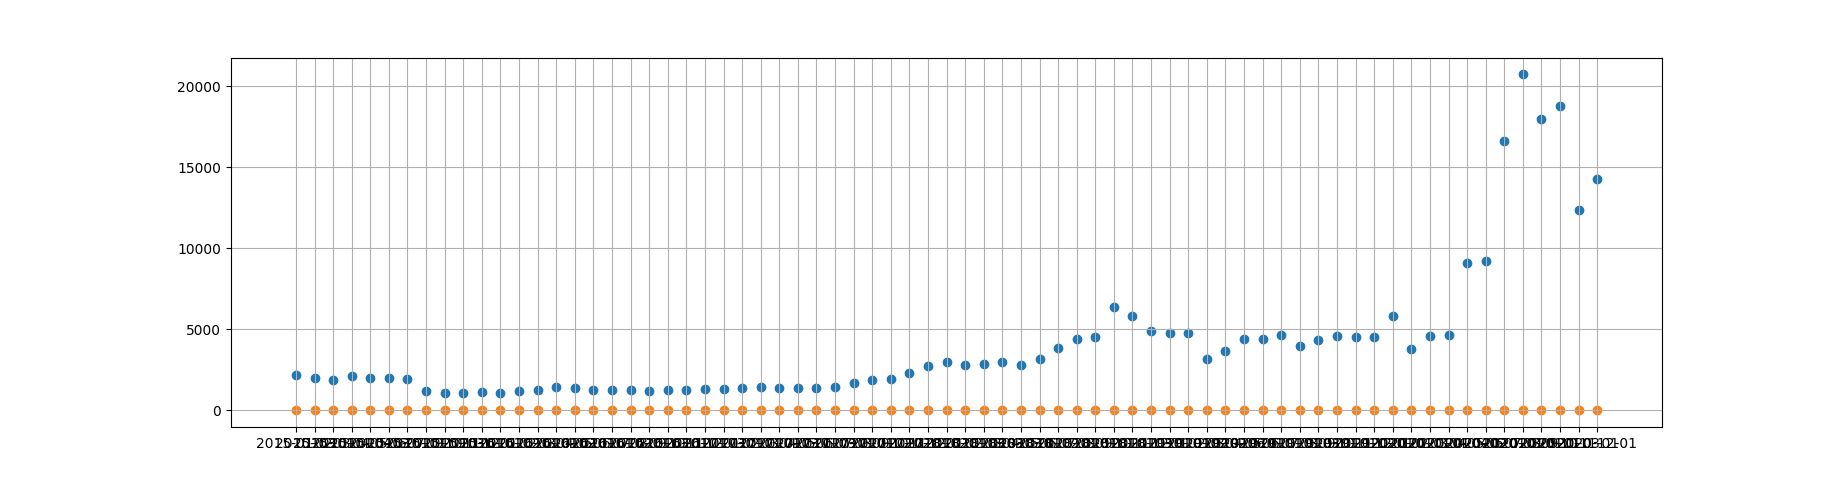
\includegraphics[width=1\textwidth] {foolad.png}
\label{foolad}$•$
\caption{
نمودار قیمت سهم فولاد
}
\end{figure}
\begin{figure}[H]
\centering
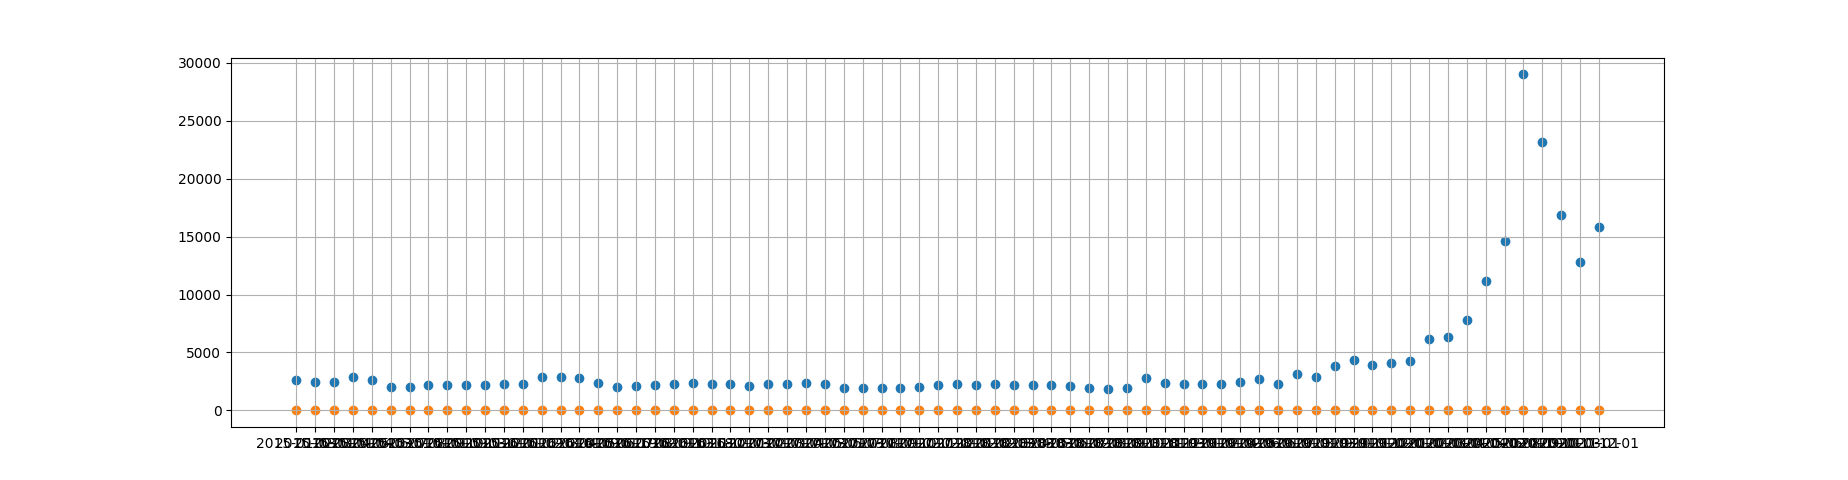
\includegraphics[width=1\textwidth] {akhaber.png}
\label{akhaber}$•$
\caption{
نمودار قیمت سهم اخابر
}
\end{figure}
همانطور که مشاهده میشود همبستگی بسیار زیاد بین قیمت دلار و قیمت نماد فولاد و نماد اخابر وجود دارد. با رسم نمودار تغییرات این دو نیز دقیقا همین به نتجیه خواهیم رسید پس از رسم مجدد آن صرف نظر میکنیم.
پس با توجه به تحلیل بالا شواهد کافی برای حضور قیمت دلار در مرحله طراحی مدل وجود دارد.


\subsubsection{بررسی تاثیر تورم}
طبق تحلیل شناختی از دیتا قابل حدس می باشد که تورم و قیمت دلار به یک معنی هستند و باید یکدیگر راتایید کنند. به منظور اطمینان بیشتر از صحت حدس خود نمودار های تغییرات دلار و تغییرات تورم را در کنار یکدیگر مورد بررسی قرار می دهیم
\begin{figure}[H]
\centering
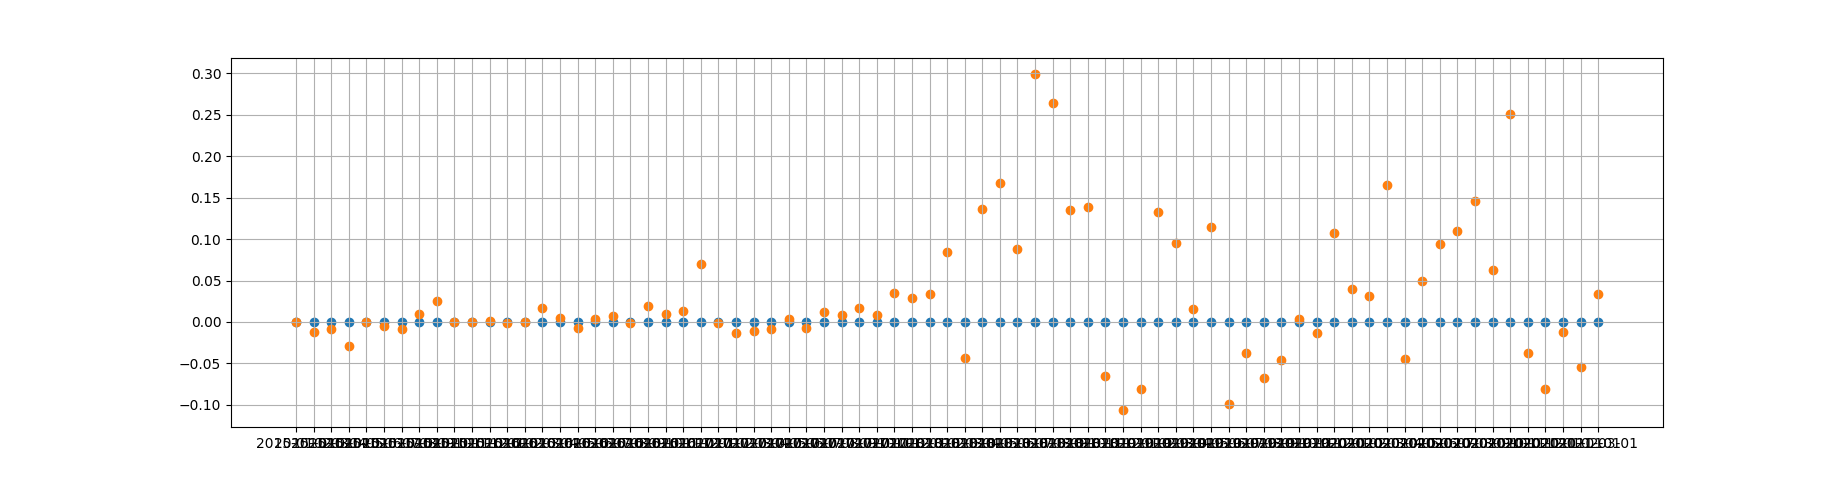
\includegraphics[width=1\textwidth] {dollar_change.png}
\label{dollar_change}$•$
\caption{
نمودار درصد تغییر قیمت دلار
}
\end{figure}
\begin{figure}[H]
\centering
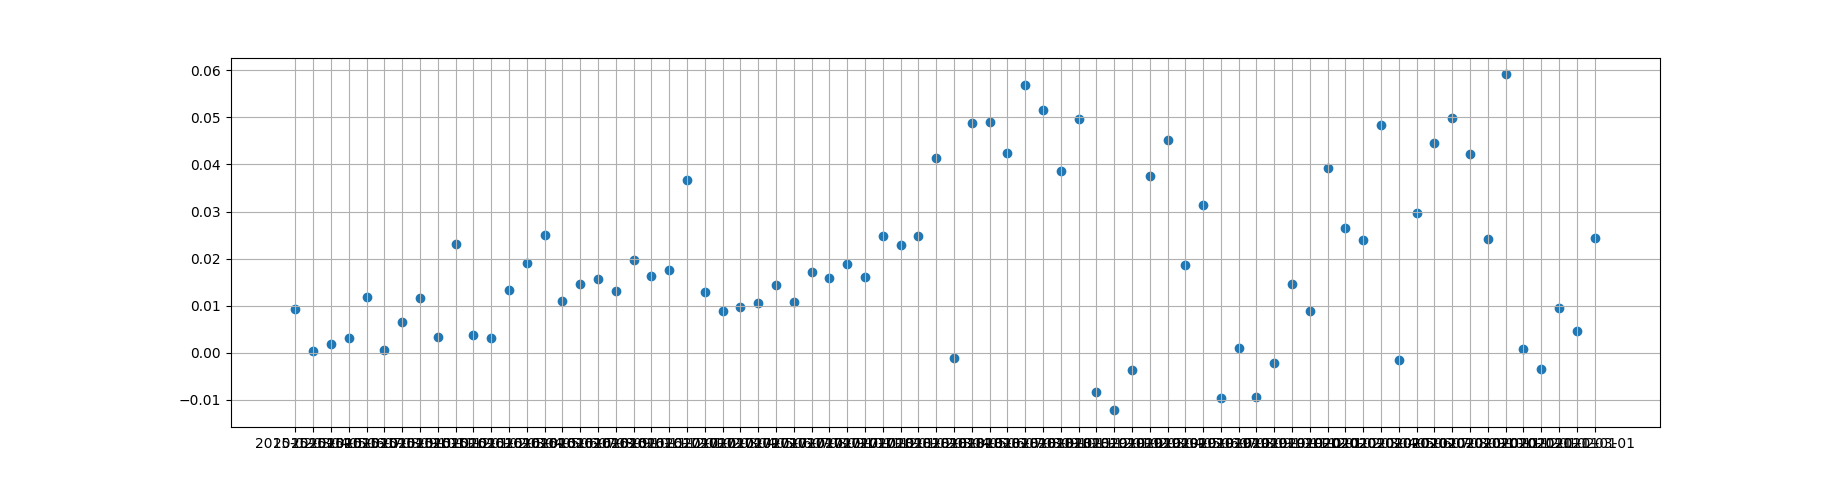
\includegraphics[width=1\textwidth] {inflation_change.png}
\label{inflation_change}$•$
\caption{
نمودار درصد تغییر تورم
}
\end{figure}
همانطور که مشاهده میشه تا حد خوبی این دو شاخص با هم همبستگی دارند ولی برای اثبات شهود خود از ضریب همبستگی پیرسون استفاده میکنیم.
طبق رابطه زیر  r رامحاسبه میکنیم
\begin{equation*}
r = \frac{\sum{(x_i-\bar{x})*(y_i-\bar{y})}}{\sqrt{\sum{(x_i-\bar{x})^2*\sum(y_i-\bar{y})^2}}}
\end{equation*}
در نهایت با محاسبه r برای دیتای  مذکور به عدد نزدیک ۱ میرسیم که نشان دهنده همبستگی مثبت خوبی هست 
با توجه به همبستگی بالای این دو شاخص میتوان از یکی آن ها در مرحله ی طراحی مدل صرف نظر کرد ولی ممکن است به هر حال یک سری اطلاعات رااز دست بدیم چون همبستگی کامل نداشتن این دو شاخص. با توجه به حجم کم دیتا شاخص تورم را نیز در مرحله ی طراحی مدل قرار می دهیم. 

\subsection{بررسی تاثیر نقدینگی}
\begin{figure}[H]
\centering
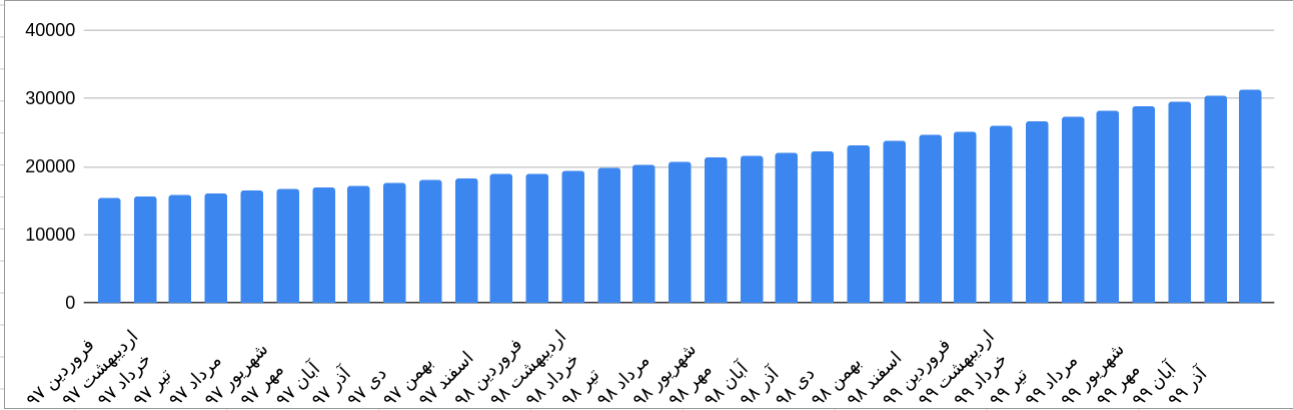
\includegraphics[width=1\textwidth] {cash.png}
\label{cash}$•$
\caption{
نمودار نقدینگی ماهانه
}
\end{figure}
با توجه به نمودار نقدینگی ماهانه متوجه میشویم که نقدینگی کاملا به صورت خطی در حال افزایش است و نوسان خاصی هم ندارد. این به این معنی هست که نقدینگی هیچ اطلاعات زیادی به ما نمیدهد. با ترسیم نمودار تغییرات نقدنگی یک خط موازی با محور x ها دریافت میکنیم و همبستگی پایینی هم بین نقدنگی و قیمت سهم ها و دلار وجود خواهد داشت. پس میتوان از ورود شاخص نقدینگی به مرحله ی مدل سازی صرف نظر کرد ولی با توجه به پیشنهاد استاد و کم بودن حجم دیتا تصمیم بر این شد که نقدینگی هم وارد مرحله مدل سازی شود.

\section{طراحی و پیاده سازی مدل}
بعد از تحلیل و انتخاب پیشگو ها با توجه به جنس  و 
خصیصه
\footnote{\lr{Feature}}
های دیتا باید به بررسی مدل های پایه و موجود بپردازیم و با استفاده از یک مدل پایه مدلی جهت پیشبینی قیمت سهم پیاده سازی کنیم.
به طور مشخص دیتا از جنس سری زمانی می باشد پس باید از بین مدل های مخصوص سری زمانی مدلی انتخاب کنیم که خصیصه های سری های زمانی را به خوبی مورد توجه قرار دهد.
\subsection{انتخاب مدل پایه}
با بررسی اولیه تمام مدل های موجود مناسب برای سری های زمانی مدل های زیر برای بررسی و تست بیشتر انتخاب شدند و مورد بررسی قرار گرفتند.
\lr{
\begin{itemize}
  \item Prophet model
  \item LSTM model
  \item ARIMA model
  \item GARCH model
\end{itemize}
}
در ادامه توضیحات بیشتری راجع به هر کدوم و دلیل رد یا انتخابشون رابیان کردیم
\subsection{مدل Prophet}
این مدل بر پایه ی
مدل افزودنی
\footnote{\lr{Additive model}}
طراحی شده است که مدلی
رگرسیونی ناپارامتری
\footnote{\lr{Nonparametric regression}}
می باشد.
این مدل بر اساس 
فصلی بودن
\footnote{\lr{seasonality}}
دیتا تصمیم میگیرد و به دنبال الگو های تکرار شونده می باشد.
بر اساس تست های اولیه ای که با این مدل گرفتیم دقت بسیار پایینی دریافت کردیم که با توجه به جمله ی قبلی خیلی دور از انتظار نبود با توجه به جنس دیتای مورد تحلیل ما.
\begin{figure}[H]
\centering
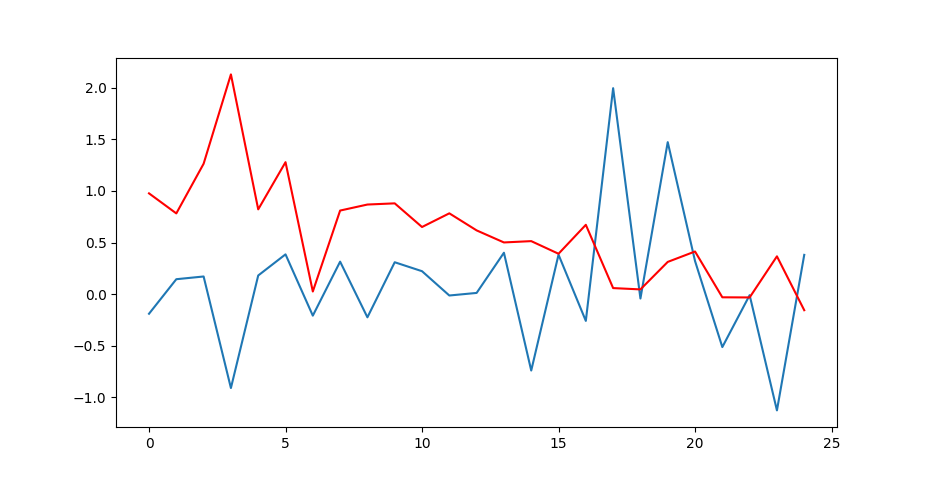
\includegraphics[width=1\textwidth] {foolad_prophet.png}
\label{foolad_prophet}$•$
\caption{
نمودار دقت مدل
}
\end{figure}
همانطور که در شکل
مشاهده می کنید، مدل خطای بالایی در پیشبینی داشته است و حتی در تشخیص 
روند
\footnote{\lr{trend}}
دچار خطا شده است و الگو رو به پایین پیشبینی کرده است. طبق محاسبه ی 
میانگین مربعات خطا
\footnote{\lr{mean squared error}}
به عدد نزدیک ۳ میرسیم که خطای بسیار زیادی میباشد.
\subsection{مدل LSTM}
این مدل بر پایه ی
شبکه ی عصبی بازگشتی
\footnote{\lr{Recurrent neural network}}
طراحی شده است و در مسائل الگو یابی کاربرد دارد از آنجایی که این مدل بسیار پیچیده است و مباحث پایه ای استفاده شده در آن خارج مباحث داده کاوی مقدماتی می باشد تلاشی برای تست این مدل به صورت عملی صورت نگرفت و صرفا در حد تحقیق باقی گذاشته شد.
\subsection{مدل ARIMA}
این مدل از ترکیب دو مدل AR یا همان
مدل خودهمبسته
\footnote{\lr{Autoregressive model}}
و
مدل میانگین متحرک
\footnote{\lr{Moving-average model}}
می باشد.
مدل خود همبسته نوعی از فرایند تصادفی می باشد و بر اساس اینکه دیتا به صورت خطی به گذشته ی خودش وابسته است کار میکند. مدل ARIMA با استفاده از ترکیب مدل AR و مدل MA ساخته شده است برای پیشبینی متغیر های پیجیده تر در سری های زمانی.
این مدل دارای ۳ پارامتر می باشد که هر کدوم به ترتیب مشخص کننده ی پارامتر مدل خودهمبسته،
درجه تفاوت
\footnote{\lr{Degree of difference}}
و درجه ی مدل میانگین متحرک می باشد.
راجع به مدل های میانگین متحرک و خودهمبسته با توجه به مربوط بودن به مباحث فرایند تصادفی و سری زمانی  خیلی در این مقاله توضیح نمیدهیم و به خواننده واگذار میکنیم. درجه تفاوت تعداد بار هایی است که باید داده با داده ی گذشته ی خود تفریق گردد تا به حالت 
ایستا
برسیم ولی با توجه به نرمال سازی دادمون و استفاده از درصد تغییرات به جای خود قیمت این پارامتر را در مدل برابر ۰ قرار میدهیم پس با این اوصاف در واقع ما داریم از مدل ARMA استفاده میکنیم.
\begin{figure}[H]
\centering
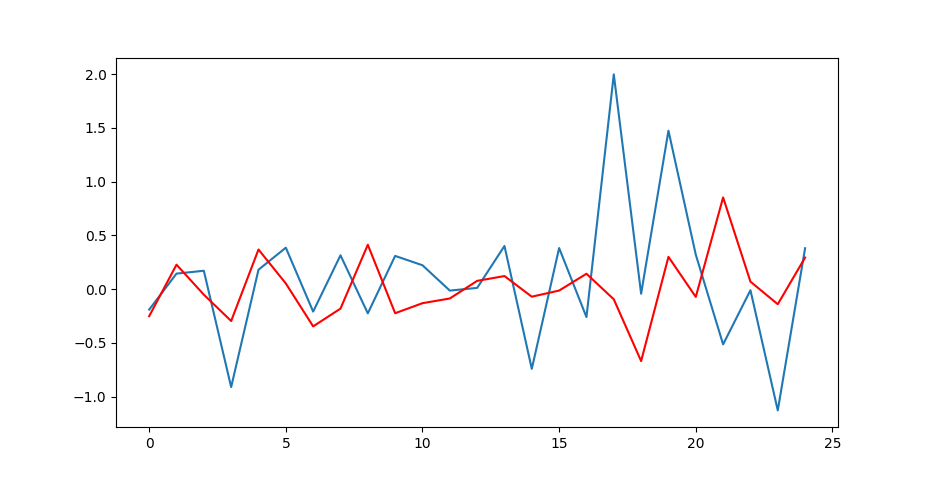
\includegraphics[width=1\textwidth] {arma1_foolad.png}
\label{arma_foolad1}$•$
\caption{
نمودار دقت مدل رو سهم فولاد
}
\end{figure}
همانطور که در شکل مشاهده میکنید دقت بسیار بیشتری بدست آماده است و مدل علاوه بر تشخیص صحیح روند اختلاف کمی با جواب اصلی دارد. خطا در این حالت حدود ۵ دهم میباشد که به نسبت مدل prophet بسیار کمتر است.
\subsection{مدل GARCH}
با توجه به نتایج خوبی که از مدل قبلی گرفتیم  این مدل را کنار گذاشتیم و مورد تست و بررسی قرار ندادیم. از آنجایی که پایه ی این مدل هم مدل خودهمبسته می باشد حدس میزدیم که نتایج بسیار متفاوتی نخواهیم گرفت. در نهایت تصمیم بر این شد که روی مدل ARMA بیشتر وقت گذاشته بشه و با تغییر پارمتر ها به بهترین دقت برسیم.

\chapter{ تحلیل نتایج و جمع بندی}
\section{نتایج بدست آمده از مدل ARIMA}
ابتدا نتایج بدست آمده از مدل رامشاهده کنیم و در آخر تحلیل نتایج راببینیم.
دو حالت برای انجام تست رو مدل امکان پذیر بود. در هر دو حالت ابتدا داده به دو قسمت آموزشی و آزمایشی تقسیم میشود که در تست های انجام شده ی ما ۶۶ درصد داده ها از ابتدای سری زمانی به عنوان داده ی آموزشی انتخاب شدند و ما بقی به عنوان داده ی آزمایشی انتخاب شدند.
حالت اول برای تست به این روش عمل میکردیم که مدل با توجه به کل داده های آزمایشی بعلاوه ی داده هایی که خودش آن ها راپیش بینی کرده آموزش داده شود و نقطه ی بعدی را پیش بینی کند و به همین ترتیب جلو برود.
حالت دوم این است که در هر مرحله عضوی که مدل پیشبینی کرده است را مقدار اصلیشو به عنوان مشاهده به مجموعه داده های آزمایشی اضافه کنیم و مدل مرحله ی بعدی را پیشبینی کند و به همین ترتیب پیش برویم.
ما در تمام تست ها از حالت اول استفاده کردیم و در بخش تحلیل بیشتر راجع به تفاوت این دو روش صحبت خواهد شد 
\subsection{نتایج عملی تست }
چند نمونه از نتایج به دست آمده توسط مدل طراحی شده در ادامه آمده است.
\begin{figure}[H]
\centering
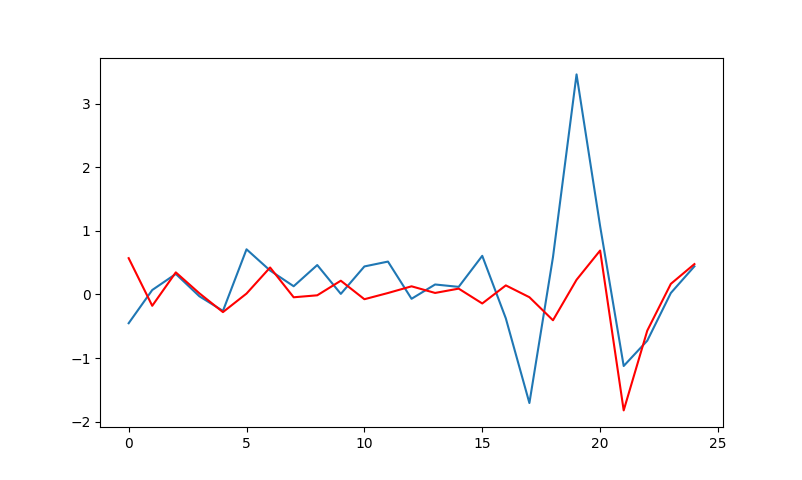
\includegraphics[width=1\textwidth] {khodro1_arima.png}
\label{khodro1_arima}$•$
\caption{
نمودار دقت مدل رو سهم خودرو با پارامتر های (۳،۰،۴)
}
\end{figure}

\begin{figure}[H]
\centering
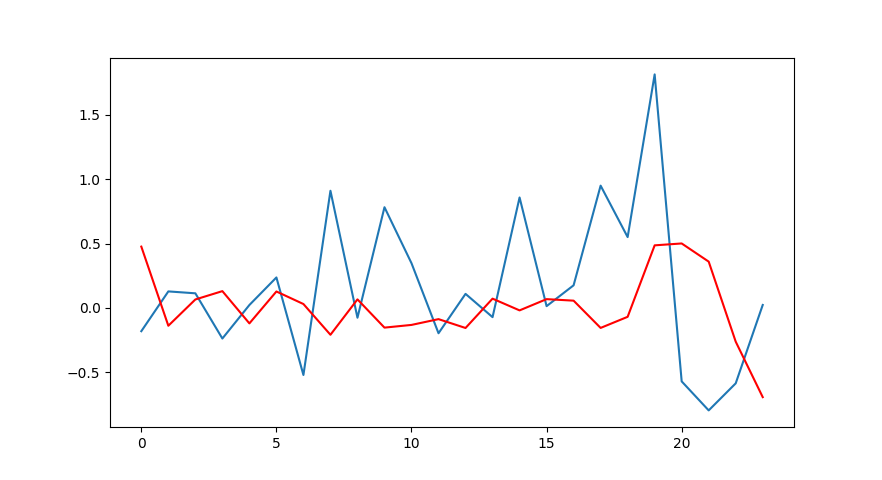
\includegraphics[width=1\textwidth] {akhaber1_arima.png}
\label{akhaber1_arima}$•$
\caption{
نمودار دقت مدل رو سهم اخابر با پارامتر های (۳،۰،۴)
}
\end{figure}

\begin{figure}[H]
\centering
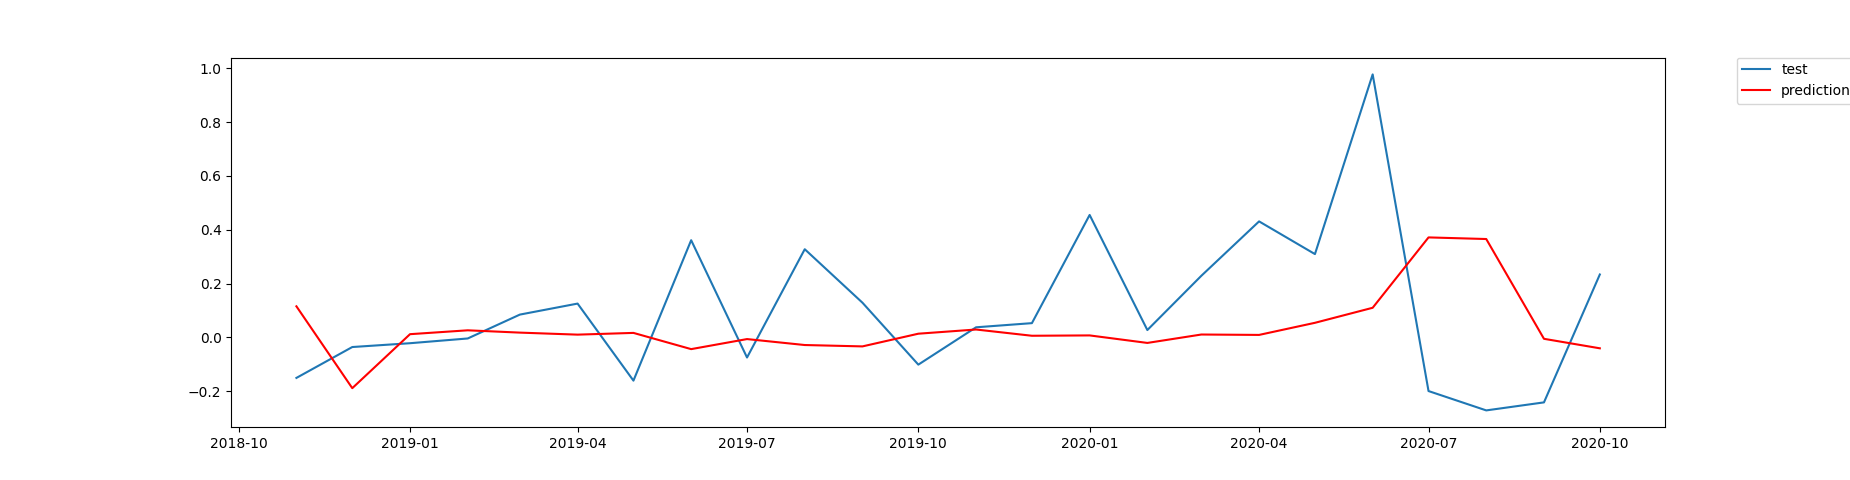
\includegraphics[width=1\textwidth] {foolad2_arima.png}
\label{foolad2_arima}$•$
\caption{
نمودار دقت مدل رو سهم اخابر با پارامتر های (۲،۰،۰)
}
\end{figure}

\subsection{تحلیل و جمع بندی}
همانطور که مشاهده می شود مدل در شروع کار دقت بهتری دارد و در ادامه رفته رفته از دقت آن کم میشود. علت این اتفاق این است که از روشی برای آزمایش و تست مدل استفاده میکنیم که پیشبینی خود مدل را به عنوان مشاهده جدید به مدل میدهیم در کنار داده های آموزشی و از آنجایی که این پیشبینی خطا دارد رفته رفته خطا به نقاط جلو تر بازنشر میشود و خطای نقاط جلوتر بیشتر میشود ولی با توجه به اینکه این روش در دنیای واقعی بیرون عملی تر و ساده تر است نسبت به روش دوم و دید بلند مدت تری ارائه می دهد ترجیح دادیم مدلمون را با توجه به این روش بهینه کنیم. 
در شکل ۳.۳ همانطور که مشاهده میکنید پارامتر مدل میانگین متحرک را برابر صفر قرار دادیم و مدل صرفا یه مدل ساده ی خودهمبسته شد و دقت نهایی کاهش پیدا کرد.
\par
در نهایت برای رسیدن به بهترین دقت با روش آزمون و خطا سعی کردیم که به بهترین پارامتر ها برای مدل برسیم ولی این روش نقطه تعادلی نداشت برامون و در نهایت مشاهده کردیم که برای هر سهم با توجه به رفتار و نوسانات بهترین دقت در پارامتر های مختلفی کسب میشود و نمیشود قانون کلی براش صادر کرد.


\chapter*{واژه‌نامه فارسی به انگلیسی}
مدل میانگین متحرک همبسته یکپارچه
\dotfill \lr{ARIMA model} \\
زبان برنامه نویسی پایتون 
\dotfill \lr{Python programming language} \\
 گیت
\dotfill \lr{Git} \\
تورم
\dotfill \lr{Predictor} \\
نقدینگی
\dotfill \lr{Asset Distribution} \\
تاریخچه قیمت
\dotfill \lr{Financial Risk} \\
قیمت پایانی
\dotfill \lr{Sharpe Ratio} \\
داده ی گم شده
\dotfill \lr{Correlation} \\
آخرین مشاهده ی انجام شده به جلو
\dotfill \lr{Eigenvalue} \\
نموداراسکتر
\dotfill \lr{Eigenvector} \\
خصیصه
\dotfill \lr{Missing Value} \\
مدل افزودنی
\dotfill \lr{Cast} \\
رگرسیون ناپارامتری
\dotfill \lr{Weight} \\
فصلی بودن
\dotfill \lr{Weight} \\
روند
\dotfill \lr{Cast} \\


\chapter*{مراجع}
\begin{latin}
[1] Larose D.T. and Larose C.D. (2014) Discovering knowledge in data: an introduction to data mining (Second edition). John Wiley \& Sons.
\newline
\newline
[2] Ruey S. Tsay, “Analysis of Financial Time Series, 3rd Edition”, WILEY, 2010.
\newline
\newline
[3] Introduction to Stochastic Processes. Lothar Breuer 
\newline
\end{latin}

\begin{latin}
\begin{abstract}
The purpose of this project is to predict the future of Tehran Stock using the history of stocks and other economic indicators such as dollar price, inflation, liquidity and etc. we tried to implement a model using data mining algorithms that can predict stock future using stock's and economic indicators history. In the first step, we collected the required data. we saved all the stocks and mentioned economic indicators from 2015 to 2020 in csv format. next step, we examined which indicators affect the stock price by drawing appropriate graphs and analyzing the indicators together then we selected the appropriate indicators. In the last step, we trained an ARIMA model to predict stock future and we tested our model.
\end{abstract}
\newpage

%Title page ---------------------------------------------
\begin{figure}
\centering
\includegraphics[height=2.5cm]{UT-Logo.pdf}
\end{figure}
\begin{center}

College of Science\\
School of Mathematics, Statistics, and Computer Science
\end{center}

\begin{center}
\huge{Analyse Iran stock exchange using data mining algorithms}
\end{center}

\begin{center}
%%%
\end{center}

\begin{center}
\textbf{
Mohammad Hossein Khoshraftar
}
\end{center}

\begin{center}
\begin{tabular}{rr}
Supervisor: & Dr. Samaneh Eftekhari Mahabadi \\

\end{tabular}
\end{center}

\vspace{3cm}
\begin{center}
A thesis submitted to Graduate Studies Office\\
in partial fulfillment of the requirements for the degree of \\
B.Sc.in\\
 Computer Science
\end{center}

\begin{center}
July , 2021
\end{center}

%\pagestyle{empty}
\pagenumbering{}

\end{latin}

\end{document}

